\chapter{Transformée de Fourier}
\label{chap:transformee}
	La décomposition en série de Fourier est un formidable outil d'analyse des signaux, mais aussi un moyen d'étude de la réponse des systèmes linéaires. Cependant, il est limité aux signaux périodiques, non bornés dans le temps. La transformée de Fourier constitue une extension de la décomposition en série de Fourier à toutes les fonctions dites apériodiques, bornées dans le temps. Dans ce chapitre, nous allons présenter de manière simple le passage de la décomposition en série de Fourier vers la transformée de Fourier, dont nous préciserons l'expression. Elle permet le passage du domaine temporel vers le domaine fréquentiel. Une transformée inverse est donc requise pour assurer le passage du domaine fréquentiel au domaine temporel : c'est le rôle de la transformée de Fourier.
	Nous préciserons les propriétés de la transformée de Fourier. Nous verrons qu'elles sont similaires non seulement à celles des séries de Fourier, mais aussi à celles de la transformée de Laplace. 
	
	\section{De la série de Fourier à la transformée de Fourier}
	Le développement en série de Fourier suppose un signal périodique. Le raisonnement que nous proposons dans cette partie va nous permettre d'étendre ce développement aux signaux apériodiques. Un signal apériodique peut être vu comme un signal périodique de période infinie. Analysons les conséquences de ce passage à l'infini sur le développement en série de Fourier et le calcul des coefficients de Fourier.
	
	Prenons le signal périodique x(t) illustré ci-dessous. Le signal est constitué d'une impulsion à durée $\Delta$ limitée, répétée tous les $n\cdot T_0$. Un développement en série de Fourier peut être réalisé pour déterminer le contenu spectral du signal. Le spectre est discret, avec une infinité d'harmoniques de la composante fondamentale à la fréquence $f_0=\frac{1}{T_0}$. L'amplitude des coefficients décroit avec la fréquence selon une enveloppe donnée.
	
	\begin{figure}[h!]
		\centering
		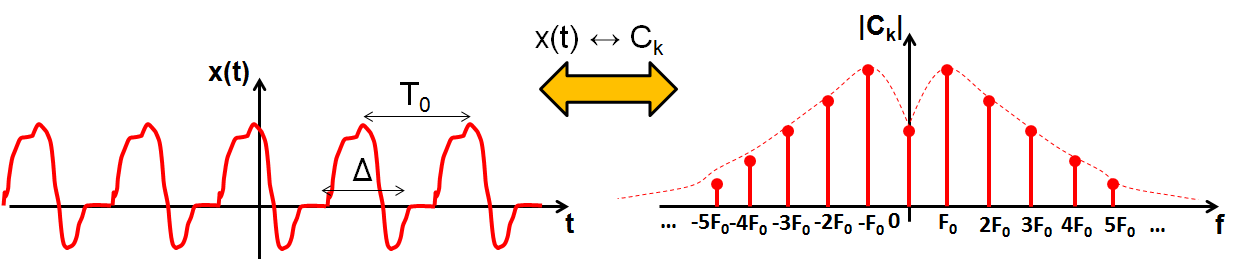
\includegraphics[scale=0.5]{images/Serie_To_Transfo_Fourier_1.png}
		\caption{Signal périodique (à gauche) et spectre (à droite)}	
		\label{Fig:Serie_To_Transfo_Fourier_1} 
	\end{figure}

	Supposons qu'on élargisse la période sans toucher à la durée $\Delta$ de l'impulsion, comme le montre la figure \ref{Fig:Serie_To_Transfo_Fourier_2}. Dans le domaine fréquentiel, les raies se rapprochent puisque la fréquence fondamentale $f_0$ a diminué. Leurs amplitudes suivent toujours la même enveloppe. Que se passe t-il si on poursuit l'augmentation de la période, en faisant tendre $T_0$ vers l'infini ? Le signal x(t) devient un signal apériodique, borné dans le temps. Dans le domaine fréquentiel, l'écart entre chaque raie s'annule et le spectre devient continu. Le spectre est donc défini à toutes les fréquences $f,~\forall~f \in \mathbb{R}$.
	
	\begin{figure}[h!]
		\centering
		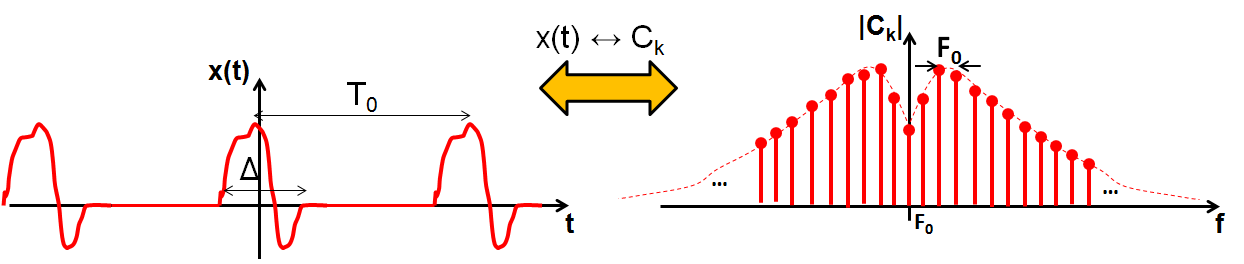
\includegraphics[scale=0.5]{images/Serie_To_Transfo_Fourier_2.png}
		\caption{Augmentation de la période du signal (à gauche) et effet sur le spectre (à droite)}	
		\label{Fig:Serie_To_Transfo_Fourier_2} 
	\end{figure}

	Un premier problème se pose : la décomposition du signal comme une somme discrète de composantes harmoniques n'est plus adaptée puisque le spectre est continu. Ce problème est facilement résolu : en faisant tendre $T_0$ vers l'infini, la somme devient une intégration. Le second problème dans le calcul des coefficients de Fourier vient du terme $\frac{1}{T_0}$, qui annule l'ensemble des coefficients de Fourier $C_k$. Une solution consiste à multiplier les coefficients de Fourier par la période $T_0$ permettant de revenir à une valeur finie. 
	En considérant ces deux modifications, et en notant $f_0 = df$ tel que $\lim_{T_0 \to +\infty}df=0$ et $kxdf=f$, on peut écrire une nouvelle formule pour calculer le spectre (\ref{Deriv_Transfo_Fourier}) en repartant de la formule de calcul des coefficients de Fourier. Comme celui-ci est continu, on le note X(f) (figure \ref{Fig:Serie_To_Transfo_Fourier_3}).
	\begin{equation}\label{Deriv_Transfo_Fourier}
	\lim_{T_0 \to +\infty}T_0\cdot C_k=\lim_{T_0 \to +\infty}T_0\cdot \int_{-\frac{T_0}{2}}^{+\frac{T_0}{2}}x(t)e^{-j2\pi kf_0 t}dt=\int_{-\infty}^{+\infty}x(t)e^{-j2\pi f t}dt=X(f)
	\end{equation}
	
	De même, on peut modifier la formule de décomposition en série de Fourier et déterminer une relation entre le signal x(t) et son spectre X(f).
	\begin{equation*}
	x(t)=\sum_{k=-\infty}^{+\infty}C_ke^{jk2\pi ft}=\sum_{k=-\infty}^{+\infty}C_k T_0 f_0 e^{jk2\pi ft}
	\end{equation*}
	\begin{equation}\label{Deriv_Transfo_Fourier_inverse}
	\lim_{T_0 \to +\infty}x(t)=\int_{-\infty}^{+\infty}X(f)e^{j2\pi f t}dt
	\end{equation}
	
	\begin{figure}[h!]
		\centering
		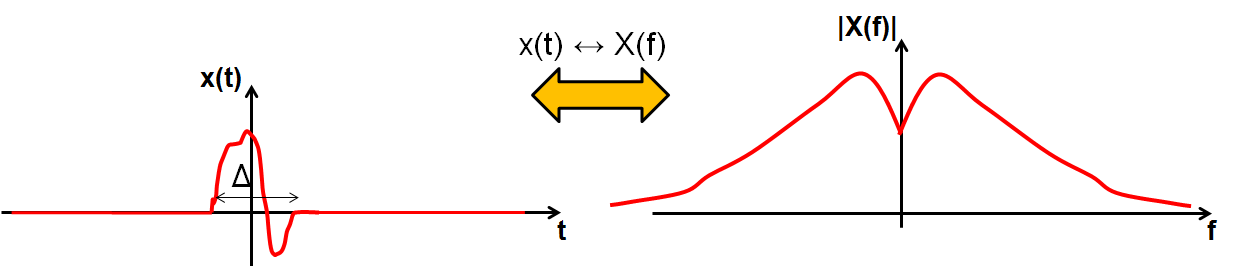
\includegraphics[scale=0.5]{images/Serie_To_Transfo_Fourier_3.png}
		\caption{Signal apériodique (à gauche) et spectre continu (à droite)}	
		\label{Fig:Serie_To_Transfo_Fourier_3} 
	\end{figure}
	
	Ces deux nouvelles relations constituent la transformée de Fourier directe (du domaine temporel au domaine fréquentiel) et inverse (du domaine fréquentiel au domaine temporel).\\ 
	
	
	
	\section{Transformées de Fourier}
	
	La transformation de Fourier constitue donc une généralisation du développement en série de Fourier pour les signaux apériodiques à support temporel borné. Elle dispose des mêmes propriétés que les séries de Fourier. On peut aussi étendre la transformée de Fourier aux signaux périodiques.
	
	L'équation \ref{Transfo_Fourier} donne l'expression de la transformée de Fourier, que l'on qualifie parfois de directe. Elle peut être vue comme un opérateur noté $\mathcal{F}$. Elle permet de calculer le spectre X(f) d'un signal temporel x(t), $\forall f \in \mathbb{R}$ et $\forall t \in \mathbb{R}$. La transformée de Fourier s'applique sur des signaux temporels à valeurs réels ou complexes. Dans ce chapitre, nous ne considérerons que des signaux temporels à valeurs réels. Par contre, le spectre X(f) est à valeurs complexes. 
	\begin{equation}\label{Transfo_Fourier}
	X(f)=\mathcal{F}[x(t)]=\int_{-\infty}^{+\infty}x(t)e^{-j2\pi f t}dt
	\end{equation}
	
	L'équation donne l'expression de la transformée de Fourier inverse, permettant de retrouver le signal temporel x(t) à partir de son spectre. Elle peut aussi être vue comme un opérateur noté $\mathcal{F}^{-1}$.
	\begin{equation}\label{Transfo_Fourier_inverse}
	x(t)=\mathcal{F}^{-1}[X(f)]=\int_{-\infty}^{+\infty}X(f)e^{+j2\pi f t}df
	\end{equation}
	
	La transformation de Fourier est bijective et unique : la transformée de Fourier de deux signaux temporels différents donnent deux spectres différents. Inversement, la transformée de Fourier inverse de deux spectres différents donne deux signaux temporels différents. 
	
	Les transformées de Fourier directe et inverse peuvent être réécrites en remplaçant la fréquences par la pulsation $\omega=2\pi f$, donnant des relations plus compactes.
	\begin{equation}\label{Transfo_Fourier_pulsation}
	X(\omega)=\int_{-\infty}^{+\infty}x(t)e^{-j\omega t}dt
	\end{equation}
	\begin{equation}\label{Transfo_Fourier_inverse_pulsation}
	x(t)=\int_{-\infty}^{+\infty}X(\omega)e^{+j\omega t}df
	\end{equation}
	 \\
	
	\underline{\textbf{Lien avec la transformée de Laplace :}}
	Lorsqu'on compare les expressions des transformées de Fourier et de Laplace bilatérale (équation \ref{Transfo_Laplace_non_causale}), on remarque que les expressions sont quasi identiques. En prenant le cas particulier où $p=j\omega$, on retrouve l'expression de la transformée de Fourier à partir de celle de Laplace. Même chose pour leur transformées inverses. 
	
	La transformation de Laplace constitue donc une généralisation de la transformation de Fourier. Les propriétés de la transformée de Laplace, vues dans le chapitre 3, se retrouveront donc lorsqu'on étudiera celles de la transformée de Fourier.\\
	
	
	
	\section{Représentation du spectre}
	
	Comme pour le développement en série de Fourier, le résultat de la transformée de Fourier peut être visualisé sous la forme d'un spectre tracé dans le domaine fréquentiel. A la différence du spectre d'un signal périodique, le spectre d'un signal apériodique est continu, donc défini pour toutes les fréquences $f \in \mathbb{R}$.
	
	Le résultat de la transformée de Fourier étant une grandeur complexe, le module et la phase sont représentées, comme l'illustre la figure \ref{Fig:Representation_spectre_Fourier}. Une représentation des parties réelles et imaginaires est aussi envisageable. Le mot spectre est généralement réservé pour la représentation de l'amplitude. En effet, il s'agit de la représentation la plus courante, car elle permet de visualiser très rapidement la distribution de l'énergie d'un signal dans le domaine fréquentiel. Cela est à l'origine d'une erreur courante. En ne représentant que l'amplitude du spectre, on omet la phase faisant du spectre une valeur réelle. Si on cherche à retrouver la forme temporelle du signal en omettant la phase, le résultat est bien entendu faussé.\\
	
	Lorsqu'on trace le spectre d'un signal x(t) périodique, l'unité de chaque raie du spectre d'amplitude est la même que le signal x(t), puisque chaque raie symbolise un terme de la décomposition en série de Fourier. Par exemple, si le signal x(t) représente l'évolution temporelle d'une tension exprimée en V, chaque raie représente une tension exprimée en V. L'unité du spectre de raies en amplitude est donc le volt dans cet exemple. Mais est-ce toujours le cas pour le spectre continu d'un signal périodique x(t) ? Est-ce que l'amplitude de son spectre $|X(f_0)|$ à une fréquence $f_0$ porte la même unité que le signal temporel ?
	
	En repartant de l'équation de la transformée de Fourier inverse (\ref{Transfo_Fourier_inverse}), on se rend compte que ça n'est pas le cas. En effet, on retrouve le signal temporel en l'intégrant sur un le domaine fréquentiel. En d'autres termes, on le retrouve en multipliant le spectre à chaque fréquence par un intervalle élémentaire de fréquence, et en sommant ces produits élémentaires. On en déduit que le spectre n'est pas homogène à l'amplitude, mais à une densité spectrale d'amplitude, soit un rapport entre l'amplitude et un intervalle de fréquence. Ainsi, lorsqu'on trace l'amplitude du spectre, on trace en fait sa densité spectrale d'amplitude. Pour alléger la tournure, on préfère parler abusivement d'amplitude. En reprenant l'exemple du signal électrique exprimé en V, la représentation de la densité spectrale d'amplitude est exprimée en V/Hz (ou en $V/rad.s^{-1}$). 
	
	\begin{figure}[h!]
		\centering
		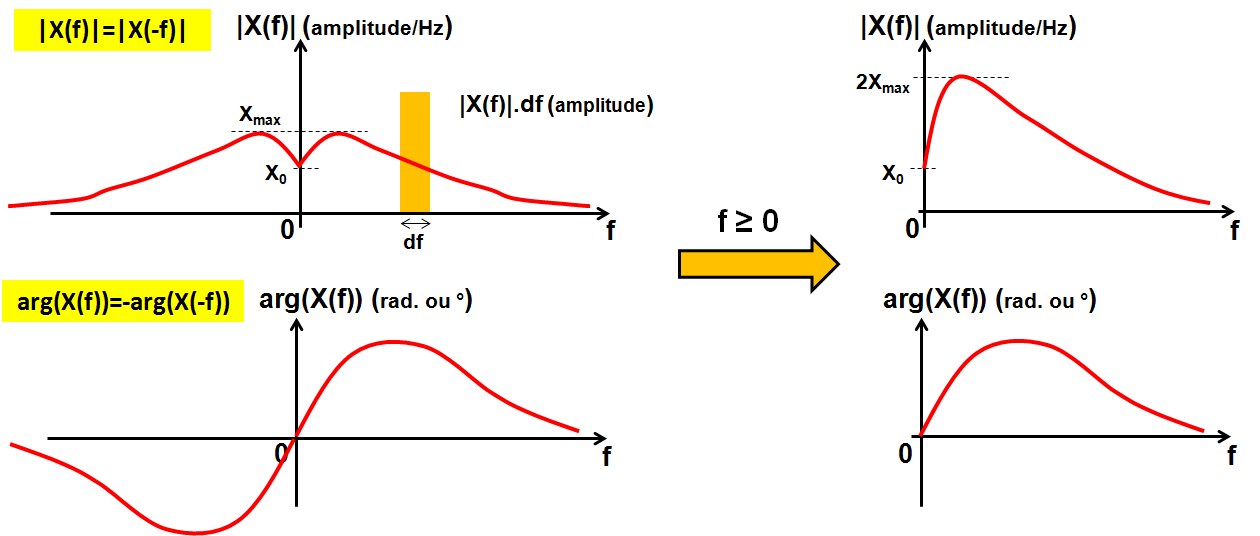
\includegraphics[scale=0.5]{images/Representation_spectre_Fourier.png}
		\caption{Représentation du spectre : symétrique (à gauche) et asymétrique (à droite)}	
		\label{Fig:Representation_spectre_Fourier} 
	\end{figure}
	
	
	On retrouve les mêmes propriétés de symétries du spectre entre les fréquences positives et négatives qu'avec la décomposition en série de Fourier. Le module est symétrique par rapport à f = 0, tandis que la phase est antisymétrique. Autrement dit, le spectre à la fréquence -f est le conjugué du spectre à la fréquence f. Leurs parties réelles sont égales, mais leurs parties imaginaires sont opposées.
	\begin{equation}\label{Symétrie_TF_module_phase}
	|X(f)|=|X(-f)|~~~~Arg(X(f))=-Arg(X(-f))
	\end{equation}
	\begin{equation}\label{Symétrie_TF_module_RI}
	X(f)=X(-f)^{*}~\Rightarrow~Re(X(f))=Re(X(-f))~~et~~Im(X(f))=-Im(X(-f))
	\end{equation}

	
	Dans le cas dx'un signal temporel à valeurs réels, la représentation que nous avons présenté est dite symétrique car elle présente le spectre sur les fréquences positives et négatives. Afin d'alléger cette représentation, il est courant de tracer une représentation asymétrique, c'est-à-dire ne représentant le spectre que pour les fréquences positives ou nulles. Elle est illustrée à la figure \ref{Fig:Representation_spectre_Fourier}.Cependant, si on conserve inchangé la densité spectrale d'amplitude et si on n'exploite que le spectre sur le domaine fréquentiel positif, on risque de diviser par deux l'amplitude du signal. Afin d'éviter toute ambiguïté, cette représentation asymétrique nécessite de doubler la densité spectrale d'amplitude (sauf en f = 0). Ainsi, en intégrant sur tout le domaine fréquentiel les densités spectrales d'amplitude des deux représentations, on retrouve la même amplitude. Pour retrouver la représentation spectrale symétrique, il faudra :
	\begin{itemize}
		\item on divise par deux le module et on le duplique du côté des fréquences négatives
		\item on duplique la phase que l'on inverse du côté des fréquences négatives.
	\end{itemize}
	Il est à noter que le même procédé aurait pu être utilisé pour une représentation spectrale asymétrique de la décomposition en série de Fourier.\\
	
	\section{Exemples de calcul de transformée de Fourier}
	
	Dans cette partie, le calcul de la transformée de Fourier est illustré à travers trois exemples de fonctions courantes.
	
	\subsection{Fonctions porte et sinus cardinal}
	La fonction porte $\pi_{\tau}(t)$, illustrée ci-dessous, est une impulsion rectangulaire de durée $\tau$ centrée en t = 0. Nous normalisons son amplitude à 1. Nous cherchons la transformée de Fourier de cette fonction, en appliquant l'équation \ref{Transfo_Fourier}.
	
	\begin{figure}[h!]
		\centering
		\includegraphics[scale=0.5]{images/Porte_Temporel.png}
		\caption{Fonction porte}	
		\label{Fig:Porte_temporel} 
	\end{figure}

	\begin{equation*}
	\Pi_{\tau}(f)=\int_{-\infty}^{+\infty}\pi_{\tau}(t)e^{-j2\pi ft}dt=\int_{-\frac{\tau}{2}}^{+\frac{\tau}{2}}1e^{-j2\pi ft}dt=\frac{1}{-j2\pi f}[e^{-j2\pi ft}]_{-\frac{\tau}{2}}^{+\frac{\tau}{2}}
	\end{equation*}
	\begin{equation*}
	\Pi_{\tau}(f)=\frac{1}{-j2\pi f}(e^{+j2\pi f\frac{\tau}{2}}-e^{-j2\pi f\frac{\tau}{2}})=\frac{sin(\pi f\tau)}{\pi f}
	\end{equation*}
	Le résultat fait apparaitre une fonction particulière appelée sinus cardinal $sinc(x)=\frac{sin(x)}{x}$, qui s'annule à chaque fois que $x=k\pi~,~k \in \mathbb{Z^{*}}$. Cette fonction est maximale en x = 0 et devient égale à 1. Le résultat de la transformée de Fourier d'une fonction porte est donc une fonction sinus cardinal tel que :
	\begin{equation}\label{TF_porte}
	\Pi_{\tau}(f)=\tau\frac{sin(\pi f\tau)}{\pi f \tau}=\tau sinc(\pi f \tau)
	\end{equation}
	Le résultat est illustré sur la figure \ref{Fig:sinc_freq}. Le spectre est purement réel. Il est maximal en f = 0 (composante continue). Il s'annule à chaque fois que  $\pi f \tau=k\pi~,~k \in \mathbb{Z^{*}}$, donc pour $f=\frac{k}{\tau}$.\\
	
	\begin{figure}[h!]
		\centering
		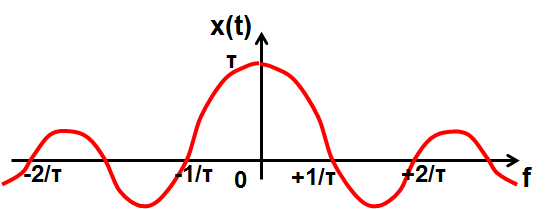
\includegraphics[scale=0.5]{images/sinc_freq.png}
		\caption{Transformée de Fourier d'une fonction porte : sinus cardinal}	
		\label{Fig:sinc_freq} 
	\end{figure}

	Ces deux fonctions sont fortement liées par la transformée de Fourier. Pour l'illustrer, considérons le spectre X(f) d'un signal qui serait borné dans le domaine fréquentiel. En notant $\frac{1}{\tau}$ la plage fréquentielle occupée par le spectre, celui-ci peut être modélisé par une fonction porte $\Pi_{\frac{1}{\tau}}(f)$. On cherche à déterminer le signal temporel x(t) qui possède un tel spectre, en calculant la transformée de Fourier inverse.
	\begin{equation*}
	x(t)=\int_{-\infty}^{+\infty}\Pi_{\frac{1}{\tau}}(f)e^{+j2\pi ft}df=\int_{-\frac{\tau}{2}}^{+\frac{\tau}{2}}e^{+j2\pi ft}df
	\end{equation*}
	\begin{equation*}
	x(t)=\frac{1}{j2\pi t \tau}[e^{+j2\pi ft}]_{-\frac{\tau}{2}}^{+\frac{\tau}{2}}=\frac{1}{\pi t \tau}\frac{e^{j\pi\frac{t}{\tau}}-e^{-j\pi\frac{t}{\tau}}}{2j}=\frac{sin(\pi\frac{t}{\tau})}{\pi t \tau}=\frac{1}{\tau}sinc(\pi\frac{t}{\tau})
	\end{equation*}
	
	Le résultat indique que la transformée de Fourier d'une fonction sinus cardinal est une fonction porte ! Il est intéressant de noter une dualité entre les domaines temporels et fréquentiels : le spectre d'un signal borné dans le temps est non borné dans le domaine fréquentiel. Inversement, un signal borné en fréquence n'est pas borné dans le domaine temporel. 
	
	\begin{figure}[h!]
			\centering
			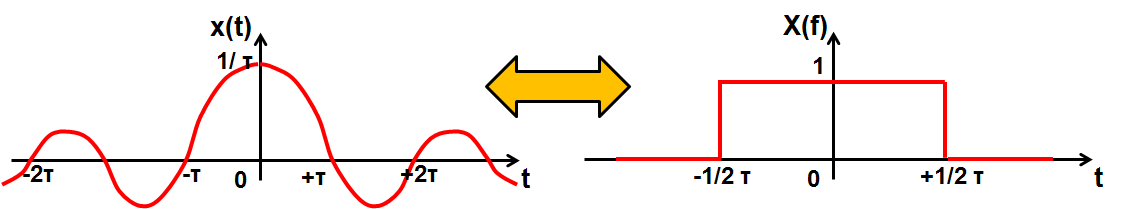
\includegraphics[scale=0.5]{images/TF_sinc.png}
			\caption{Transformée de Fourier d'une fonction sinus cardinal : une fonction porte}	
			\label{Fig:TF_sinc} 
	\end{figure}
	
	
	
	\subsection{Impulsion de Dirac}
	L'impulsion de Dirac n'est certes pas une fonction (c'est une distribution), mais on peut calculer sa transformée de Fourier. 
	\begin{equation}\label{key}
	\mathcal{F}(\delta(t))=\int_{-\infty}^{+\infty}\delta(t) e^{-j2\pi ft}dt = e^{-j2\pi f0}=1
	\end{equation}
	La transformée de Fourier d'une impulsion de Dirac est constant et égal à 1. Le spectre est donc uniforme quelle que soit la fréquence, correspondant à un signal "blanc". Il rejoint la remarque faite précédemment sur la dualité entre des signaux bornés dans le temps et bornés en fréquence. La durée de l'impulsion de Dirac est infiniment brève. Il en résulte un spectre infiniment large !\\
	Ce résultat est conforme à la définition de l'impulsion de Dirac, dont l'amplitude est infinie. La valeur '1' correspond à une densité spectrale d'amplitude. Pour revenir à l'amplitude du signal, il faudrait intégrer cette valeur sur tout le domaine fréquentiel, conduisant à une amplitude infinie.\\
	
	On peut aussi s'intéresser à la transformée de Fourier inverse d'une impulsion de Dirac, centrée sur une fréquence $f_0$. Une telle distribution se note $\delta(f-f_0)$. Elle indique un spectre dont toute la densité spectrale d'amplitude est concentrée en un point de fréquence $f_0$. L'amplitude du signal temporel associé sera donc finie et il pourra être représentée par une fonction. On peut cependant remarquer qu'un tel spectre ne peut être celui d'un signal réel, puisque le spectre n'est pas symétrique. Le résultat, indiqué ci-dessous, le confirme : la transformée de Fourier inverse d'une impulsion de Dirac est une exponentielle complexe. Dans le cas où l'impulsion de Dirac est centrée en f=0, le spectre redevient symétrique et correspond à celui d'un signal continu égal à 1.
	\begin{equation}\label{key}
	\mathcal{F}(\delta(f-f_0))=\int_{-\infty}^{+\infty}\delta(f-f_0) e^{+j2\pi ft}df=e^{+j2\pi f_0 t}
	\end{equation}
	
	
	
	
	\subsection{Fonctions cosinus et sinus}
	
	De prime abord, la transformée de Fourier d'une fonction sinusoïdal ou cosinusoïdal ne semble pas une question compliquée. Comme il s'agit de fonctions périodiques, on peut les développer en séries de Fourier. Celles-ci ne sont constitués que de la composante harmonique fondamentale. On s'attend donc à ce que la transformée de Fourier de ces fonctions puissent être représentée par deux impulsions de dirac, centrées en $f_0$ et en $-f_0$.
	
	Cependant, si on applique la transformée de Fourier à une fonction (co)sinusoïdale, on arrive à une difficulté de calcul sérieuse. Prenons l'exemple d'une fonction cosinusoïdale et appliquons l'opérateur transformée de Fourier. Le cosinus peut être développé sous la forme de deux exponentielles complexes :
	\begin{equation*}
	\mathcal{F}[cos(\omega_{0}t)]=\int_{-\infty}^{+\infty}cos(\omega_{0}t)e^{-j\omega t}dt=\int_{-\infty}^{+\infty}\frac{e^{j\omega_{0}t}+e^{-j\omega_{0}t}}{2}e^{-j\omega t}dt
	\end{equation*}
	\begin{equation*}
	\mathcal{F}[cos(\omega_{0}t)]=\int_{-\infty}^{+\infty}\frac{e^{j(\omega_{0}-\omega)t}+e^{-j(\omega_{0}+\omega)t}}{2}dt
	\end{equation*}
	
	Il nous faut intégrer deux termes exponentiels complexes sur l'ensemble des réels, sachant que ces fonctions ne convergent pas vers une valeurs finie lorsque t tend vers l'infini. La résolution de ces intégrales n'est pas triviale et nécessite la mise en œuvre de concepts mathématiques qui dépassent le cadre de ce cours.
	
	Une solution, plus simple, consiste à utiliser le résultat de la partie précédente, qui nous à montrer que la transformée de Fourier d'une exponentielle complexe, de fréquence $f_0$, est l'impulsion de Dirac $\delta(f-f_0)$. Puisque la fonction cosinus est la superposition de deux exponentielles complexes, de fréquence $f_0$ et $-f_0$, on peut facilement en déduire la transformée de Fourier d'une fonction cosinusoïdale :
	\begin{equation}\label{key}
	\mathcal{F}[cos(2\pi f_0 t)]=	\mathcal{F}[\frac{e^{j2\pi f_0 t}+e^{-j2\pi f_0 t}}{2}]=\frac{1}{2}	\mathcal{F}[e^{j2\pi f_0 t}]+\frac{1}{2}\mathcal{F}[e^{-j2\pi f_0 t}]=\frac{\delta(f-f_0)}{2}+\frac{\delta(f+f_0)}{2}
	\end{equation}  
	
	De même, on peut en déduire celle d'une fonction sinusoïdale :
	\begin{equation}\label{key}
	\mathcal{F}[sin(2\pi f_0 t)]=	\mathcal{F}[\frac{e^{j2\pi f_0 t}-e^{-j2\pi f_0 t}}{2j}]=\frac{1}{2j}	\mathcal{F}[e^{j2\pi f_0 t}]-\frac{1}{2j}\mathcal{F}[e^{-j2\pi f_0 t}]=\frac{\delta(f-f_0)}{2j}-\frac{\delta(f+f_0)}{2j}
	\end{equation}  
	
	Le spectre de ces deux fonctions est représenté sur la figure \ref{Fig:TF_cos_sin} .
	
	\begin{figure}[h!]
		\centering
		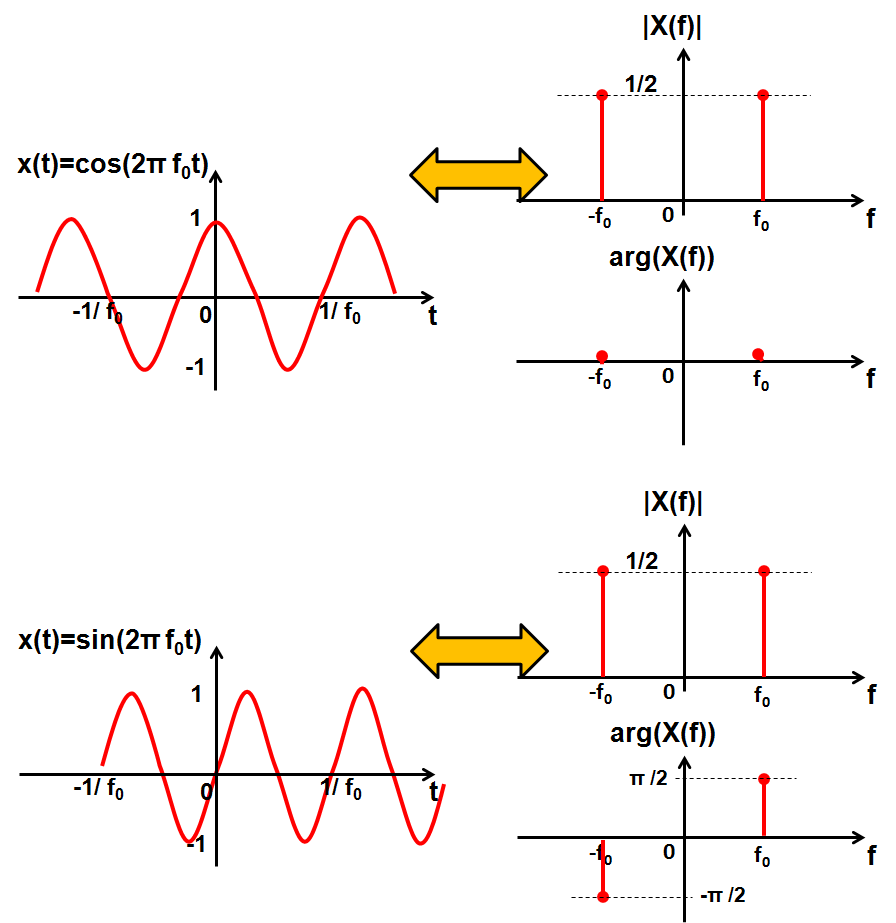
\includegraphics[scale=0.4]{images/TF_cos_sin.png}
		\caption{Transformée de Fourier des fonctions cosinus et sinus}	
		\label{Fig:TF_cos_sin} 
	\end{figure}
	
	
	
	
	
	\section{Propriétés de la transformée de Fourier}
	On retrouve les même propriétés que pour la décomposition en série de Fourier et la transformée de Laplace. Le tableau \ref{Tab:Propriétés_Transfo_Fourier} récapitule les propriétés principales.
	
	\begin{table}[h!]
		\centering
		\caption{\label{Tab:Propriétés_Transfo_Fourier} Tableau récapitulatif des propriétés de la transformée de Fourier}
		\begin{tabular}{|l|c|}
			\hline
			Linéarité & $ax(t)+by(t)~\Leftrightarrow~aX(f)+bY(f)$ \\	
			\hline
			Théorème du retard & $x(t-t_0)~\Leftrightarrow~X(f)e^{-j2\pi f t_0}$ \\	
			\hline
			Théorème du changement d'échelle $y(t)=x(at)$ & $Y(f)=\frac{1}{|a|}X(\frac{f}{|a|})$ \\	
			\hline
			Dérivée temporelle & $y(t)=\frac{d^{k}x(t)}{dt^{k}}~\Leftrightarrow~Y(f)=(j2\pi f)^{k}X(f)$ \\
			\hline
			Dérivée fréquentielle & $Y(f)=\frac{d^{k}X(f)}{df^{k}}~\Leftrightarrow~y(t)=(-j2\pi t)^{k}x(t)$ \\
			\hline
			Intégration temporelle & $y(t)=\int_{-\infty}^{t}x(\tau)d\tau~\Leftrightarrow~Y(f)=\frac{1}{2}X(0)\delta(f)+\frac{X(f)}{j2\pi f}$ \\
			\hline
			Produit de convolution dans le domaine temporel & $y(t)=x_1*x_2 (t)~\Leftrightarrow~Y(f)=X_1(f)\cdot X_2(f)$ \\
			\hline
			Dualité & si $x(t)~\Leftrightarrow~X(f)$ alors $ X(t)~\Leftrightarrow~x(-f)$ \\
			\hline
			Produit de convolution dans le domaine fréquentiel & $y(t)=x_1 \cdot x_2 (t)~\Leftrightarrow~Y(f)=X_1* X_2(f)$ \\
			\hline
		\end{tabular}	
	\end{table}
	
	\section{Table de transformée de Fourier courante}
	Le tableau \ref{Tab:Transfo_Fourier_usuelles} récapitule les transformées de Fourier de fonctions courantes.
	
	\begin{table}[h!]
		\centering
		\caption{\label{Tab:Transfo_Fourier_usuelles} Tableau récapitulatif des propriétés de la transformée de Fourier}
		\begin{tabular}{|l|c|}
			\hline
			\textbf{Domaine temporel} & \textbf{Domaine fréquentiel} \\
			\hline
			Fonction porte $x(t)=\pi_{\tau}(t)$ & $X(f)=\tau sinc(\pi f \tau)$ \\	
			\hline
			Sinus cardinal $x(t)=\frac{1}{\tau} sinc(\pi \frac{t}{\tau})$  & $X(f)=\Pi_{\frac{1}{\tau}}(f)$ \\	
			\hline
			Fonction triangle $x(t)=	\left \{
			\begin{array}{l}
			1-\frac{|t|}{\tau}~si~|t|<\tau \\
			0~sinon \\
			\end{array}
			\right .$  & $X(f)=sinc(\pi \frac{t}{\tau})^{2}$ \\	
			\hline
			Impulsion de Dirac $\delta(t)$ & 1 \\	
			\hline
			Cosinus $\cos(2\pi f_0 t)$ & $\frac{e^{j2\pi f_0 t}+e^{-j2\pi f_0 t}}{2}$ \\	
			\hline
			Sinus $\sin(2\pi f_0 t)$ & $\frac{e^{j2\pi f_0 t}-e^{-j2\pi f_0 t}}{2j}$ \\	
			\hline
			Fonction signe $x(t)=sgn(t)=\frac{t}{|t|}$ & $X(f)=\frac{1}{j\pi f}$ \\	
			\hline
			Echelon de Heaviside $x(t)=u(t)$ & $X(f)=\frac{1}{j2\pi f} + \frac{\delta(f)}{2}$ \\	
			\hline
			$x(t)=\alpha e^{-\alpha t}u(t)$ & $X(f)=\frac{\alpha}{\alpha+j2\pi f}$ \\	
			\hline
			$x(t)=\frac{\alpha}{2} e^{-\alpha |t|}$ & $X(f)=\frac{\alpha^{2}}{\alpha^{2}+(2\pi f)^{2}}$ \\	
			\hline
			$x(t)=\alpha{2}te^{-\alpha |t|}u(t)$ & $X(f)=\frac{\alpha^{2}}{(\alpha+j2\pi f)^{2}}$ \\	
			\hline
			$x(t)=e^{-\alpha t}cos(2 \pi f_0 t)u(t)$ & $X(f)=\frac{\alpha+j2\pi f}{(\alpha+j2\pi f)^{2}+(2\pi f_0)^{2}}$ \\	
			\hline
			$x(t)=e^{-\alpha t}sin(2 \pi f_0 t)u(t)$ & $X(f)=\frac{2\pi f_0}{(\alpha+j2\pi f)^{2}+(2\pi f_0)^{2}}$ \\	
			\hline
		\end{tabular}	
	\end{table}
	
	
	\section{Excitation d'un système linéaire par un signal périodique}
	Lorsqu'un signal x(t) excite un système linéaire à temps invariant, sa réponse peut être facilement déterminée à partir de sa transformée de Fourier de l'excitation. C'est ce qu'illustre la figure \ref{Fig:Excitation d'un système linéaire par un signal apériodique}. En effet, en raison des propriétés de linéarité de la transformée de Fourier, la réponse y(t) sera égale à celle-ci, mais pondérée par la fonction de transfert du système H. Cette propriété offre un moyen alternatif à la transformée de Laplace pour calculer la réponse d'un système linéaire.
	\begin{equation}\label{key}
	y(t)=\mathcal{F}^{-1}[Y(f)]=\mathcal{F}^{-1}[H(f)X(f)]
	\end{equation}
	
	\begin{figure}[h!]
		\centering
		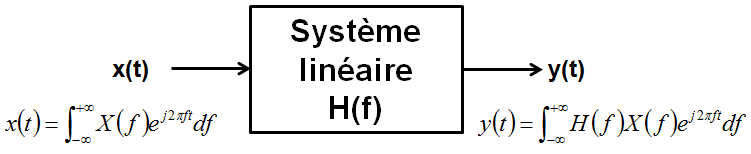
\includegraphics[scale=0.6]{images/LTI_TF.png}
		\caption{Exemple de représentation du spectre de raies en amplitude (en haut) et en phase (en bas)}	
		\label{Fig:Excitation d'un système linéaire par un signal apériodique} 
	\end{figure}
	
	
	
	\section{Exercices}
	
	\subsubsection{Exercice 1}
	
	On considère le signal $s_1$ défini pour tout réel t par :
	\begin{equation*}
	s_1(t)=e^{-at}u(t)
	\end{equation*}
	où u(t) est la fonction échelon de Heaviside et $a \in \mathbb{R_{+}^{*}}$. Tracez le graphe de $s_1$. Déterminez sa transformée de Fourier $S_1$.\\
	
	2. En utilisant les propriétés de la transformée de Fourier, déterminer après avoir tracé le graphe des signaux $s_2$ et $s_3$ :
	
	a. la transformée de Fourier $S_2$ du signal $s_2$ défini pour tout réel t par $s_2(t)=e^{at}u(-t)$.\\
	
	b.la transformée de Fourier $S_3$ du signal $s_3$ défini pour tout réel t par $s_2(t)=e^{-a|t|}$.\\
	
	c. la transformée de Fourier $S_4$ du signal $s_4$ défini pour tout réel t par $s_4(t)=-e^{at}u(-t)+e^{-at}u(t)$.\\
	
	\subsubsection{Exercice 2}
	
	Calculez les transformées de Fourier de signaux suivants :\\
	
	a. $v(t) = cos(2\pi f_0 t)\pi_{T_0}(t)$\\
	
	b. $w(t) = \delta(t-T_e)+\delta(t)+\delta(t+T_e)$\\
	
	c. $x(t) = \delta(t-2T_e)+\delta(t)+\delta(t+2T_e)$\\
	
	d. $x(t) = te^{-at}u(t)~,~~a>0$\\
	
	e. La fonction y(t) décrite sur la figure \ref{Fig:Exo_TF_2}.
	
	\begin{figure}[h!]
		\centering
		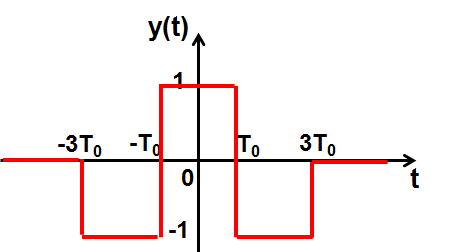
\includegraphics[scale=0.5]{images/exo_2_TF.png}
		\caption{Figure exercice 2}	
		\label{Fig:Exo_TF_2} 
	\end{figure}
	
	
	\subsubsection{Exercice 3 - Signal numérique}
	On considère l'impulsion de forme trapézoïdale présentée sur la figure \ref{Fig:Exo_TF_3}. Celle-ci constitue un modèle simplifié des signaux électriques numériques.
	
	\begin{figure}[h!]
		\centering
		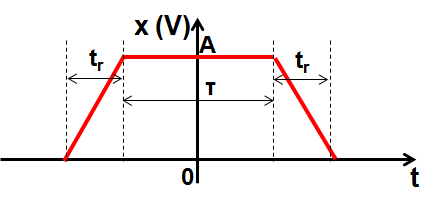
\includegraphics[scale=0.6]{images/exo_3_TF.png}
		\caption{Figure exercice 3}	
		\label{Fig:Exo_TF_3} 
	\end{figure}

	1. Calculez la transformée de Fourier du signal.\\
	
	2. Esquissez l'allure de son spectre (module seulement). Précisez l'unité.\\
	
	3. Calculez l'énergie de ce signal.\\
	
	4. Le spectre est-il à bande limitée ? Quelle(s) paramètre(s) affectent l'occupation spectrale du signal ?\\
	

	
	\subsubsection{Exercice 4}
	Soit un filtre passe-bas RC, avec R = 1 k$\Omega$ et C = 1 $\mu$F. On envoie en entrée un signal $x(t)=e^{-10^{3}t}u(t)$.\\
	
	1. Etablir la fonction de transfert du filtre en fonction de la fréquence.\\
	
	2. Calculez la transformée de Fourier X(f) du signal x(t).\\
	
	3. Déterminez le spectre de la réponse du filtre.\\
	
	4. Calculez la réponse du filtre dans le domaine temporel.\\